\documentclass[../main/Notes.tex]{subfiles}
\begin{document}

\section[Solution 6: Signal Detection Theory xxxBut which number to put here?xxx]{Solution 6: Signal Detection Theory I+II \iftoggle{showdates}{\small{\textit{2014-06-27}}}{}}

\subsection*{Excercise 4}\index{Low Threshold Theory}\label{sheet6ex4}

Luce's idea is: If High Threshold Theory does not work, maybe by using a low threshold, ROC curves will be explainable. This idea translates as follows:

\begin{align*}
S \in \{ y,n \} , D \in \{ y,n \} , R \in \{ y,n \} \\
P\left(D=y|S=y\right) = p_{y} \\
P\left(D=y|S=n\right) = p_{n} > 0
\end{align*}

We have to consider to different cases of the subject's behaviour.

\textbf{Case 1:} The subject want to lower his false-alarm rate $p(FA)$:
\begin{align*}
& P\left(R=y|D=n\right) = 0 \\
& P\left(R=y|D=y\right) = t < 1\\
\Rightarrow P(FA) & = P\left(R=y|D=y\right) &\cdot~& P\left(D=y|S=n\right) &+~&P\left(R=y|D=n\right)&\cdot~ & P\left(D=n|S=n\right) \\
& = t &\cdot~& p_{n} &+~& 0 &\cdot~& \left(1-p_{n}\right) \\
& = t \cdot~ p_{n} \\
\Rightarrow P(H) & = P\left(R=y|D=y\right) &\cdot~& P\left(D=y|S=y\right) &+~&P\left(R=y|D=n\right)&\cdot~ & P\left(D=n|S=y\right) \\
& = t &\cdot~& p_{y} &+~& 0 &\cdot~& \left(1-p_{y}\right) \\
& = t \cdot~ p_{y} \\
& = \frac{P(FA)}{p_{n}} \cdot~ p_{y}
\end{align*}

Now the first part of the plot looks like this:
\begin{figure}[ht!]
  \centering
  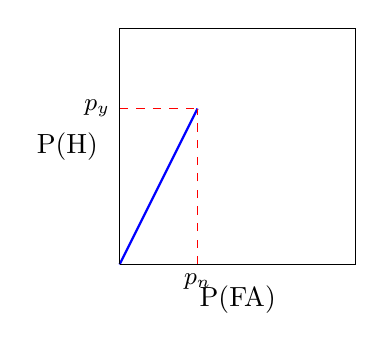
\begin{tikzpicture}[scale=3]
  \node[below] at (0.33,0) {\small $p_{n}$};
  \node[left] at (0,0.66) {\small $p_{y}$};
    \node[below] at (0.5,-0.05) {P(FA)};
  \node[left] at (-0.05,0.5) {P(H)};
  \draw[thick, blue] (0,0) -- (0.33,0.66);
  \draw[dashed, red] (0.33,0) -- (0.33,0.66);
   \draw[dashed, red] (0,0.66) -- (0.33,0.66);
   	\draw (0,0) -- (0,1) --(1,1) -- (1,0) -- (0,0);
  \end{tikzpicture}
  \caption{Low Threshold Model, first part of plot with slope of $\frac{p_{y}}{p_{n}}$}
  \label{fig:2014-06-27_firstPartLowThrsh}
\end{figure}

\textbf{Case 2:} The subject wants a higher hit rate $p(H)$:
\begin{align*}
& P\left(R=y|D=Y\right) = 1 \\
& P\left(R=y|D=n\right) = u > 0\\
\Rightarrow P(FA) & = P\left(R=y|D=y\right) &\cdot~& P\left(D=y|S=n\right) &+~&P\left(R=y|D=n\right)&\cdot~ & P\left(D=n|S=n\right) \\
& = 1 &\cdot~& p_{n} &+~& u &\cdot~& \left(1-p_{n}\right) \\
& = p_{n} + u \cdot~ \left(1-p_{n}\right)\\
\Leftrightarrow u &= \frac{P(FA)-p_{n}}{1-p_{n}} \\
\Rightarrow P(H) & = P\left(R=y|D=y\right) &\cdot~& P\left(D=y|S=y\right) &+~&P\left(R=y|D=n\right)&\cdot~ & P\left(D=n|S=y\right) \\
& = 1 &\cdot~& p_{y} &+~& u &\cdot~& \left(1-p_{y}\right) \\
& = p_{y} +  u \cdot~  \left(1-p_{y}\right)\\
& = p_{y} +  \frac{P(FA)-p_{n}}{1-p_{n}} \cdot~  \left( 1-p_{y} \right)\\
& = \frac{1-p_{y}}{1-p_{n}} \cdot~ P(FA) + \frac{p_{y}-p_{n}}{1-p_{n}}
\end{align*}

We can finish our plot:
\begin{figure}[ht!]
  \centering
  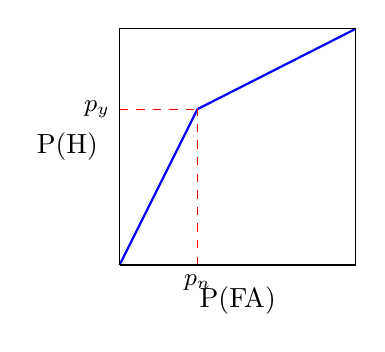
\begin{tikzpicture}[scale=3]
  \node[below] at (0.33,0) {\small $p_{n}$};
  \node[left] at (0,0.66) {\small $p_{y}$};
    \node[below] at (0.5,-0.05) {P(FA)};
  \node[left] at (-0.05,0.5) {P(H)};
  \draw[thick, blue] (0,0) -- (0.33,0.66);
   \draw[thick, blue] (0.33,0.66) -- (1,1);
  \draw[dashed, red] (0.33,0) -- (0.33,0.66);
   \draw[dashed, red] (0,0.66) -- (0.33,0.66);
   	\draw (0,0) -- (0,1) --(1,1) -- (1,0) -- (0,0);
  \end{tikzpicture}
  \caption{Low Threshold Model Plot}
  \label{fig:2014-06-27_LowThrshPlot}
\end{figure}

As can be seen, Low Threshold Theory better fits the actual data since its form is, compared with the linear function of High Threshold Theory, more like that of an ROC curve. Nevertheless it is not the right model for what is really going on.

\end{document}